\documentclass[letterpaper]{article}
\usepackage{aaai24}  % Update to the latest AAAI style file
\usepackage{times}
\usepackage{helvet}
\usepackage{courier}
\usepackage[hyphens]{url}
\usepackage{hyperref}
\usepackage{graphicx}
\urlstyle{rm}
\def\UrlFont{\rm}
\usepackage{natbib}
\usepackage{caption}
\frenchspacing
\setlength{\pdfpagewidth}{8.5in}
\setlength{\pdfpageheight}{11in}

% These packages are optional, remove if not needed
\usepackage{algorithm}
\usepackage{algorithmic}
\usepackage{newfloat}
\usepackage{listings}

\usepackage{hyperref}

\usepackage{amsmath}

\usepackage{caption}
\usepackage{subcaption}

\DeclareCaptionStyle{ruled}{labelfont=normalfont,labelsep=colon,strut=off}
\lstset{
    basicstyle={\footnotesize\ttfamily},
    numbers=left,numberstyle=\footnotesize,xleftmargin=2em,
    aboveskip=0pt,belowskip=0pt,
    showstringspaces=false,tabsize=2,breaklines=true
}
\floatstyle{ruled}
\newfloat{listing}{tb}{lst}{}
\floatname{listing}{Listing}

\usepackage{xcolor}
\newcommand{\todo}[1]{{\color{orange}{TODO: #1}}}
\newcommand{\gur}[1]{{\color{teal}{Gur: #1}}}
\newcommand{\naomi}[1]{{\color{magenta}{Naomi: #1}}}

% Update the title and author information
\title{Learning to Estimate Search Progress Using Graph Neural Networks \thanks{This work expands on \citet{sudry2022learning}.}}
\author{
    Gur Keinan\textsuperscript{\rm 1},
    Naomi Derel\textsuperscript{\rm 1}
}
\affiliations{
    \textsuperscript{\rm 1}Technion - Israel Institute of Technology\\
    gur.keinan@campus.technion.ac.il, naomi.derel@campus.technion.ac.il
}

\pdfinfo{
/TemplateVersion (2023.1)
}

\begin{document}

\maketitle

\begin{abstract}
    Estimating search progress in heuristic search algorithms remains a crucial challenge in automated planning and problem-solving. While previous approaches have derived formulas of progress estimation, and further work has shown promise in learning to predict search progress, these methods overlook the structural information embedded in the search graph created by the search algorithm. 
    We propose a novel approach using Graph Neural Networks (GNNs) to leverage this valuable structural information for more accurate search progress estimations. By representing the search space as a graph where nodes correspond to expanded states and edges to state transitions, the GNN can learn meaningful patterns in the search trajectory, which indicate progress toward the goal. 
    Using multiple domain-related and general heuristic functions, we evaluate our approach on two distinct domains, Blocks-World and Sliding-Window Puzzle. This diversity in problem spaces allows us to assess the model's generalization ability across different search problems. 
    Our results demonstrate that a GNN-based approach can effectively capture search patterns and provide more accurate progress estimates compared to previous methods. This improvement holds both in unseen problem instances and across different domains, whether on complete search graphs or intermediate ones observed throughout the search.
    This suggests that incorporating structural information through GNNs leads to more robust and generalizable search progress estimation, potentially improving the efficiency of heuristic search algorithms in practical applications.
\footnote{The materials of this project are available on \href{https://github.com/GurKeinan/Artificial-Intelligence-and-Autonomous-Systems}{GitHub}.}
\end{abstract}

\section{Introduction}

Many real-world problems can be effectively modeled within classical search spaces and tackled using well-established heuristic search algorithms. The task of accurately predicting search progress is essential in several practical applications.
Beyond simply estimating completion time, accurate progress prediction allows better resource allocation, informs algorithm selection, and plays a vital role in temporal planning. In temporal planning scenarios \citep{cashmore2018temporal}, where actions have durations and deadlines, the ability to estimate remaining search time helps prioritize promising search paths that are more likely to yield timely solutions.

Classic approaches to predicting search progress have primarily relied on predefined functions based on limited features. These traditional methods are limited in their expressive power and ability to adapt to the dynamic nature of different search spaces. 

% \naomi{cite or remove - Statistical approaches, such as those using pattern databases or sampling techniques, provide more flexibility but can be computationally intensive and may struggle with generalization across diverse problem domains.}

More recent works have tried to leverage machine learning methods for this task, like the LSTM-based approach introduced in \citet{sudry2022learning}. This approach represented a substantial advance by learning directly from search behavior, and allows for fine-tuning heuristic and domain-specific characteristics. However, these methods are restricted by treating search nodes as sequential data points, failing to capture the full structural relationships inherent in the search space. This limitation can result in less accurate progress predictions, particularly in complex or large-scale search problems.

Our work builds on this idea by integrating graph neural networks to capture and explicitly leverage the structure of the search space, learning over the graph formed by algorithms like A* \citep{hart1968formal}. This approach is novel in enabling the model to learn from both the features of individual nodes and the relationships between them. The underlying intuition is that this structural awareness supports more nuanced predictions by considering the broader context of the search process.

In this work, we aim to validate the effectiveness of our approach, investigating its capacity to enhance search progress predictions through structural insights. We developed a comprehensive framework for creating and analyzing search graphs of varying sizes and difficulties from classical planning problems, with a focus on 2 domains: Blocks-World and Sliding-Puzzle. These generated problem instances were solved using A* search with multiple domain-based and general heuristics, and the generated search trees were saved as graph structures. Our framework captures rich information about both the structure of the search graph, as well as rich node features such as heuristic values, depth in the search tree, branching factors, and various search progress indicators as introduced by \citet{sudry2022learning}.

We propose two primary GNN models: a heavier architecture and a more lightweight one. To assess their performance, we performed extensive experiments in various domains and at different search progress checkpoints. Our GNN models significantly outperformed previous approaches, reducing mean squared error (MSE) by an order of magnitude compared to both traditional formula-based estimators and a Random Forest (RF) model. More importantly, our models demonstrated strong generalization capabilities. When trained on one domain and tested on another, they maintained high performance with only a modest drop in accuracy—comparable to previous methods' performance when tested within the same training domain.

These findings suggest that our GNN-based approach captures fundamental patterns in search behavior that are transferable across problem types. Additionally, our lightweight architecture achieved comparable or better performance than its more complex counterpart, indicating that the structural information captured by GNNs is more meaningful than architectural sophistication for this task.

\subsection{Our Contribution}

Our work offers four key contributions:
\begin{enumerate}
    \item A novel approach for estimating search progress using graph neural networks, significantly outperforming previous sequence-based approaches.
    \item A comprehensive framework for constructing and collecting search graphs from classical planning problems, incorporating flexible problem generators, multiple heuristics, and pruning.
    \item Two distinct GNN architectures, optimized for different computational requirements.
    \item Empirical demonstration of strong cross-domain generalization, showing an order of magnitude improvement in prediction accuracy over traditional methods even when generalizing to unseen domains.
\end{enumerate}

\section{Background}

In this section we briefly review the necessary background for heuristic search, our goal of search progress estimation, and the GNN architecture.

\subsection{Planning Problems and Heuristic Search}

A planning problem is formally represented as a state-space search problem, defined by a tuple $T = \langle S, S_0, S_g, A, f, c\rangle$, where: $S$ is the finite set of all possible states, $S_0$ is the initial state, $S_g$ is the set of goal states, $A(s)$ represents the set of actions applicable in state $s$, $f: S \times A \rightarrow S$ is the state transition function mapping a state and action to a resultant state, and $c(s,a)$ is the cost function for action $a$ performed from state $s$.

To solve planning problems efficiently, heuristic search algorithms like A* use a heuristic function $h(s)$ that estimates the cost from any state $s$ to a goal state. A* maintains an open list of nodes to explore, ordering them by $f(s) = g(s) + h(s)$, where $g(s)$ is the known cost from the initial state to $s$. The algorithm expands nodes by generating their successors until reaching a goal state or exhausting the search space.

\subsection{Search Progress Estimation}

When solving a heuristic search problem, estimating the search progress of the last expanded node helps predict how much longer it will take to find a solution. Following \cite{sudry2022learning}, we define search progress formally.

Let $A$ be a search algorithm, and $P$ be a heuristic search problem. Define $E_A(P)$ as the total nodes expanded by $A$ when solving $P$, and $Gen_A(P)$ as the number of nodes currently expanded. The remaining nodes to be expanded is $Rem_A(P, Gen_A(P)) = E_A(P) - Gen_A(P)$.

The search progress at any point is then defined as:
\begin{equation*}
    Prog_A(P) = \frac{Gen_A(P)}{Gen_A(P) + Rem_A(P, Gen_A(P))}
\end{equation*}

This measure ranges from 0 to 1, representing the fraction of the total search effort already expended. The challenge lies in estimating $Rem_A(P, Gen_A(P))$ while the search is still in progress, as the total number of nodes to be expanded is unknown until a solution is found.

\subsection{Graph Neural Networks}
Graph Neural Networks (GNNs) are deep learning models designed to operate on graph-structured data \citep{scarselli2008graph}. In their most general form, GNNs learn node representations through iterative message passing between nodes, aggregating information from their local neighborhoods. 

Formally, for a node $v$ with features $h_v$, its representation is updated through a message passing process:
\begin{equation*}
    h_v^{(l+1)} = \text{UPDATE}(h_v^{(l)}, \text{AGG}(\{m_{u\rightarrow v}^{(l)} : u \in \mathcal{N}(v)\}))
\end{equation*}
where $m_{u\rightarrow v}^{(l)}$ represents messages from neighboring nodes, $\mathcal{N}(v)$ denotes the neighborhood of node $v$, and $l$ indicates the layer.

Two prominent GNN variants are Graph Convolutional Networks (GCN) and Graph Attention Networks (GAT). 

GCNs \citep{kipf2016semi} use a weighted sum for aggregation:
\begin{equation*}
    h_v^{(l+1)} = \sigma \left( W^{(l)} \sum_{u \in \mathcal{N}(v)} \frac{1}{\sqrt{|\mathcal{N}(u)|\cdot|\mathcal{N}(v)|}} \cdot h_u^{(l)} \right)
\end{equation*}
where $W^{(l)}$ is a learnable weight matrix and $\sigma$ is a nonlinear activation.

Expanding upon this, GATs \citep{velivckovic2017graph} introduce attention mechanisms to weight neighbor contributions:
\begin{equation*}
    h_v^{(l+1)} = \sigma \left( \sum_{u \in \mathcal{N}(v)} \alpha_{vu} W^{(l)} h_u^{(l)} \right)
\end{equation*}
Attention coefficients $\alpha_{vu}$ can be computed as:
\begin{equation*}
    \alpha_{vu} = \frac{\exp(\text{LeakyReLU}(a^T[W \cdot h_v \| W \cdot h_u]))}{\sum_{k \in \mathcal{N}(v)} \exp(\text{LeakyReLU}(a^T[W \cdot h_v \| W \cdot h_k]))}
\end{equation*}
where LeakyReLU is a non-linear activation function and $\|$ is the concatenation operator.

Modern GNN architectures enhance these base models with several key components. 

Layer normalization stabilizes training by normalizing node features within each layer, using learnable parameters to maintain model expressiveness. 

Residual connections allow direct gradient flow by adding a node's previous representation to its transformed features, helping prevent degradation in deeper networks. 

Multi-head attention runs parallel attention mechanisms, each potentially capturing different aspects of node relationships, with outputs typically concatenated or averaged. 

These components can be complemented by learnable edge weights and improved aggregation schemes, allowing the model to better capture the importance of different node relationships and structural patterns in the graph. Together, these elements enable more robust and expressive GNN architectures while maintaining stable training dynamics.


\subsection{Related Work}

Previous approaches to search progress estimation can be broadly categorized into offline and online methods. 

\paragraph{Offline methods} attempt to predict search effort before the search begins by analyzing the search space structure. 

\citet{breyer2008recent} focused on predicting A* node expansions for the 15-puzzle, developing analytical formulas based on pattern database statistics. 
\citet{lelis2014estimating} introduced a more general approach using sampling to estimate search tree size, where they performed random walks in the search space to estimate branching factors and solution depth. \citet{hutter2014algorithm} proposed methods for algorithm runtime prediction using instance features and machine learning, though this focused on overall runtime rather than progress during search. \citet{kilby2006estimating} showed that by weighting branches according to their probability of being visited during random probing, and by using recursive assumptions about search tree symmetry, search tree size could be estimated effectively without advance knowledge of the tree structure.

\paragraph{Online methods} make predictions during the search process using information from expanded nodes. \citet{thayer2012we} introduced several influential estimators:

The Velocity-based Search Progress (VeSP) estimator calculates search \emph{velocity} as:
\begin{equation*}
    V = \frac{h_0 - h_{min}}{Gen_A(P)}
\end{equation*}
where $h_0$ is the initial state's heuristic value and $h_{min}$ is the minimum heuristic value seen so far. It then estimates remaining search effort as $SE_V = h_{min}/V$, leading to the progress estimate:
\begin{equation}
    VeSP(Gen_A(P)) = \frac{Gen_A(P)}{Gen_A(P) + SE_V}
\end{equation}

The Vacillation-based Search Progress (VaSP) estimator improves upon VeSP by incorporating expansion delay - the average number of expansions between when a node is generated and when it is expanded. Using $\Delta e$ to denote \emph{expansion delay}, it estimates remaining effort as:
\begin{equation*}
    SE_e = \Delta e \times h_{min}
\end{equation*}
yielding the progress estimate:
\begin{equation}
    VaSP(Gen_A(P)) = \frac{Gen_A(P)}{Gen_A(P) + SE_e}
\end{equation}

The Path-based Progress (PBP) estimator takes a different approach by looking at the ratio between path cost and estimated total cost. For a node $n$, it calculates:
\begin{equation}
    NPBP(n) = \frac{g(n)}{g(n) + h(n)}
\end{equation}
where $g(n)$ is the cost to reach $n$ and $h(n)$ is the heuristic estimate. The final PBP estimate is the maximum NPBP value among expanded nodes.

\paragraph{Learning to Estimate:}\label{para:learning-to-estimate}
The work of \citet{sudry2022learning} marked a significant shift by applying deep learning to this problem. Their LSTM-based approach processes sequences of expanded nodes, representing a significant shift towards applying deep learning to search progress estimation. For each node, they capture basic search node-features and global features:

\begin{itemize} 
    \item $g(n)$ - cost to reach the node
    \item $h(n)$ - heuristic estimate
    \item $f(n)$ - total estimated cost
    \item $b(n)$ - branching factor
    \item $N(n)$ - node serial number
    \item $h_0$ - initial heuristic value
    \item $h_{min}$ - minimum h-value seen
    \item $N_{h_{min}}$ - number of nodes since the last $h_{min}$ update
    \item $f_{max}$ - maximum f-value seen
\end{itemize}

Their results demonstrated that this learned approach could outperform hand-crafted estimators across various domains, particularly in handling the complex patterns that emerge during the search.

\paragraph{Graph Neural Networks in Planning:} GNNs have been successfully applied to various aspects of planning and search algorithms. \citet{toyer2020asnets} introduced Action Schema Networks (ASNets), which learn generalized policies for PDDL planning problems by exploiting their relational structure and can generalize from small training instances to larger problems. \citet{chen2024learning} developed graph representations for learning domain-independent heuristics, notably introducing a method that operates directly on lifted representations of planning tasks. \citet{staahlberg2022learning} employed a simplified GNN architecture for learning generalized policies in classical planning, establishing connections between GNN expressiveness and first-order logic fragments. \citet{9636442} demonstrated GNNs' utility in continuous search spaces by integrating them with Monte Carlo Tree Search for motion planning in autonomous driving. These diverse applications highlight GNNs' capability to effectively process and learn from structured planning and search spaces.

\paragraph{GNNs for Progress Estimation:} While GNNs have been widely applied to various graph-based tasks, their use for search progress estimation remains largely unexplored.
While LSTMs capture temporal patterns in the sequence of expanded nodes, they don't explicitly model the structural relationships in the search space. GNNs can directly operate on the graph structure of expanded nodes, where edges represent state transitions. This allows the model to learn from both node features and the topological structure of the search space, potentially enabling more accurate predictions by leveraging this additional structural information.

\section{Data}

\begin{figure*}[ht]
    \centering
    \begin{minipage}{0.57\textwidth} % Two-thirds width
        \centering
        \caption*{Overlap in Block-World Instances}
        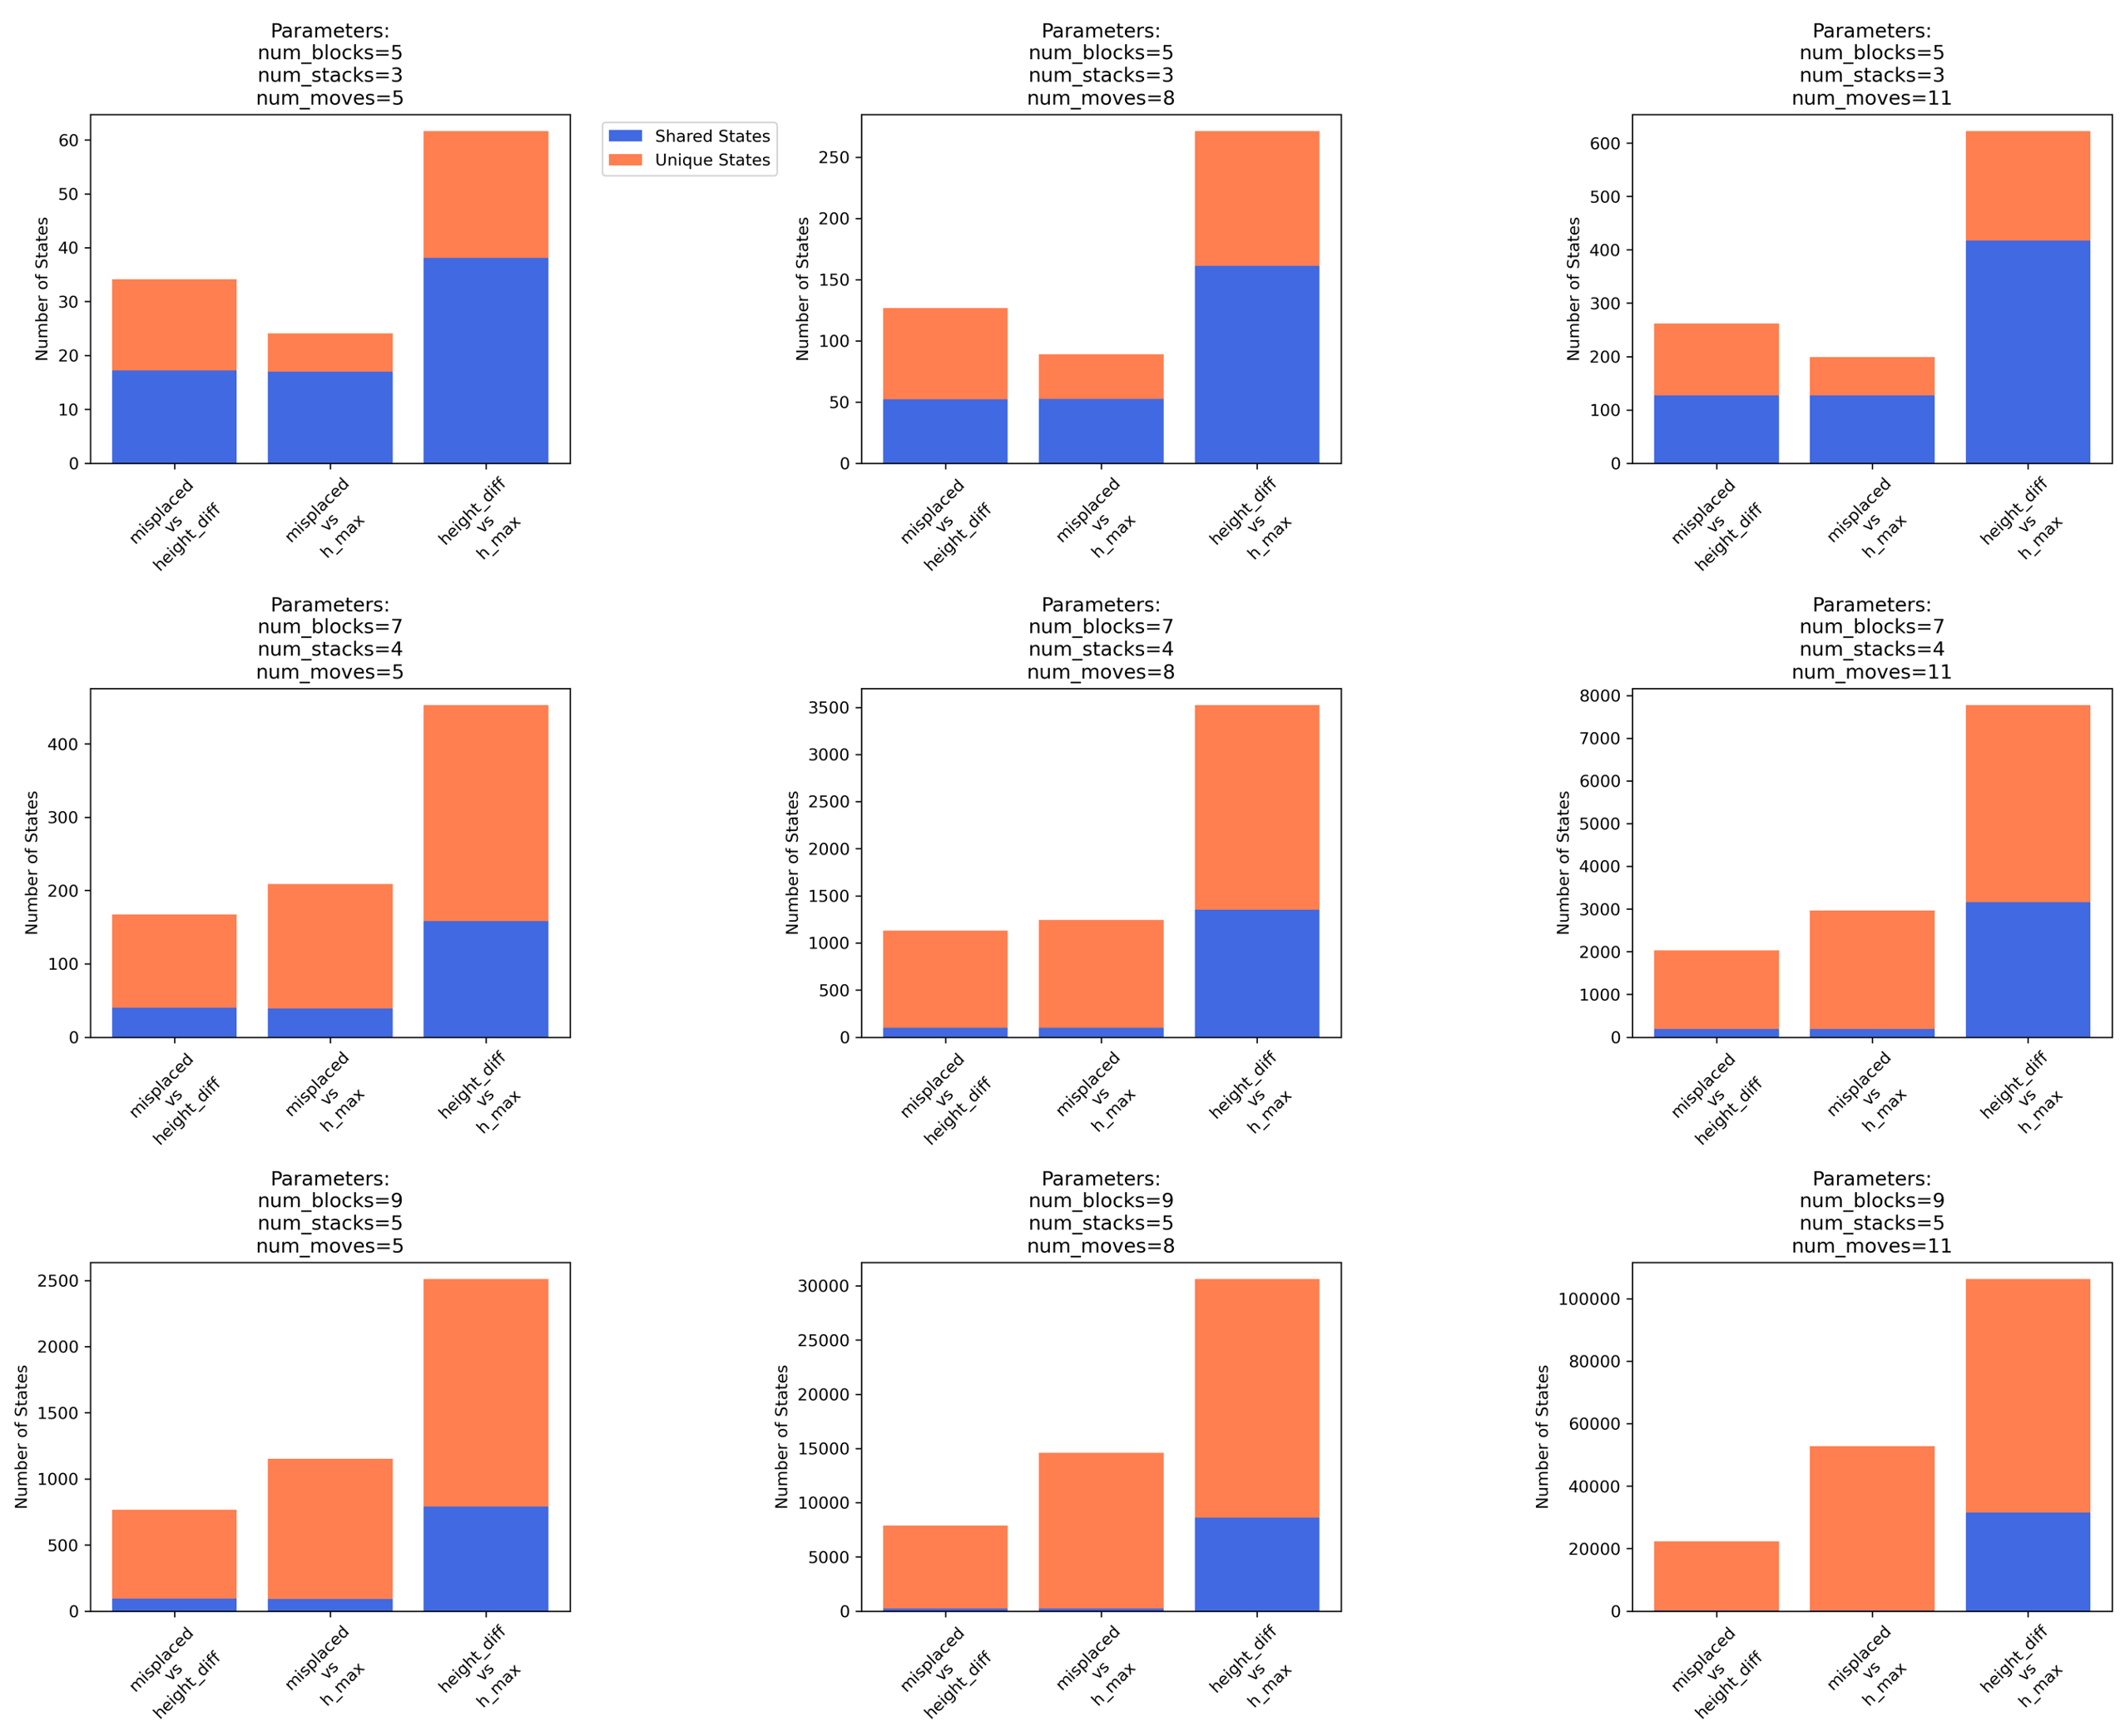
\includegraphics[width=\textwidth]{plots/blocks_world_state_overlap_2.png}
    \end{minipage}%
    \hfill
    \begin{minipage}{0.39\textwidth} % One-third width
        \centering
        \caption*{Overlap in Sliding-Puzzle Instances}
        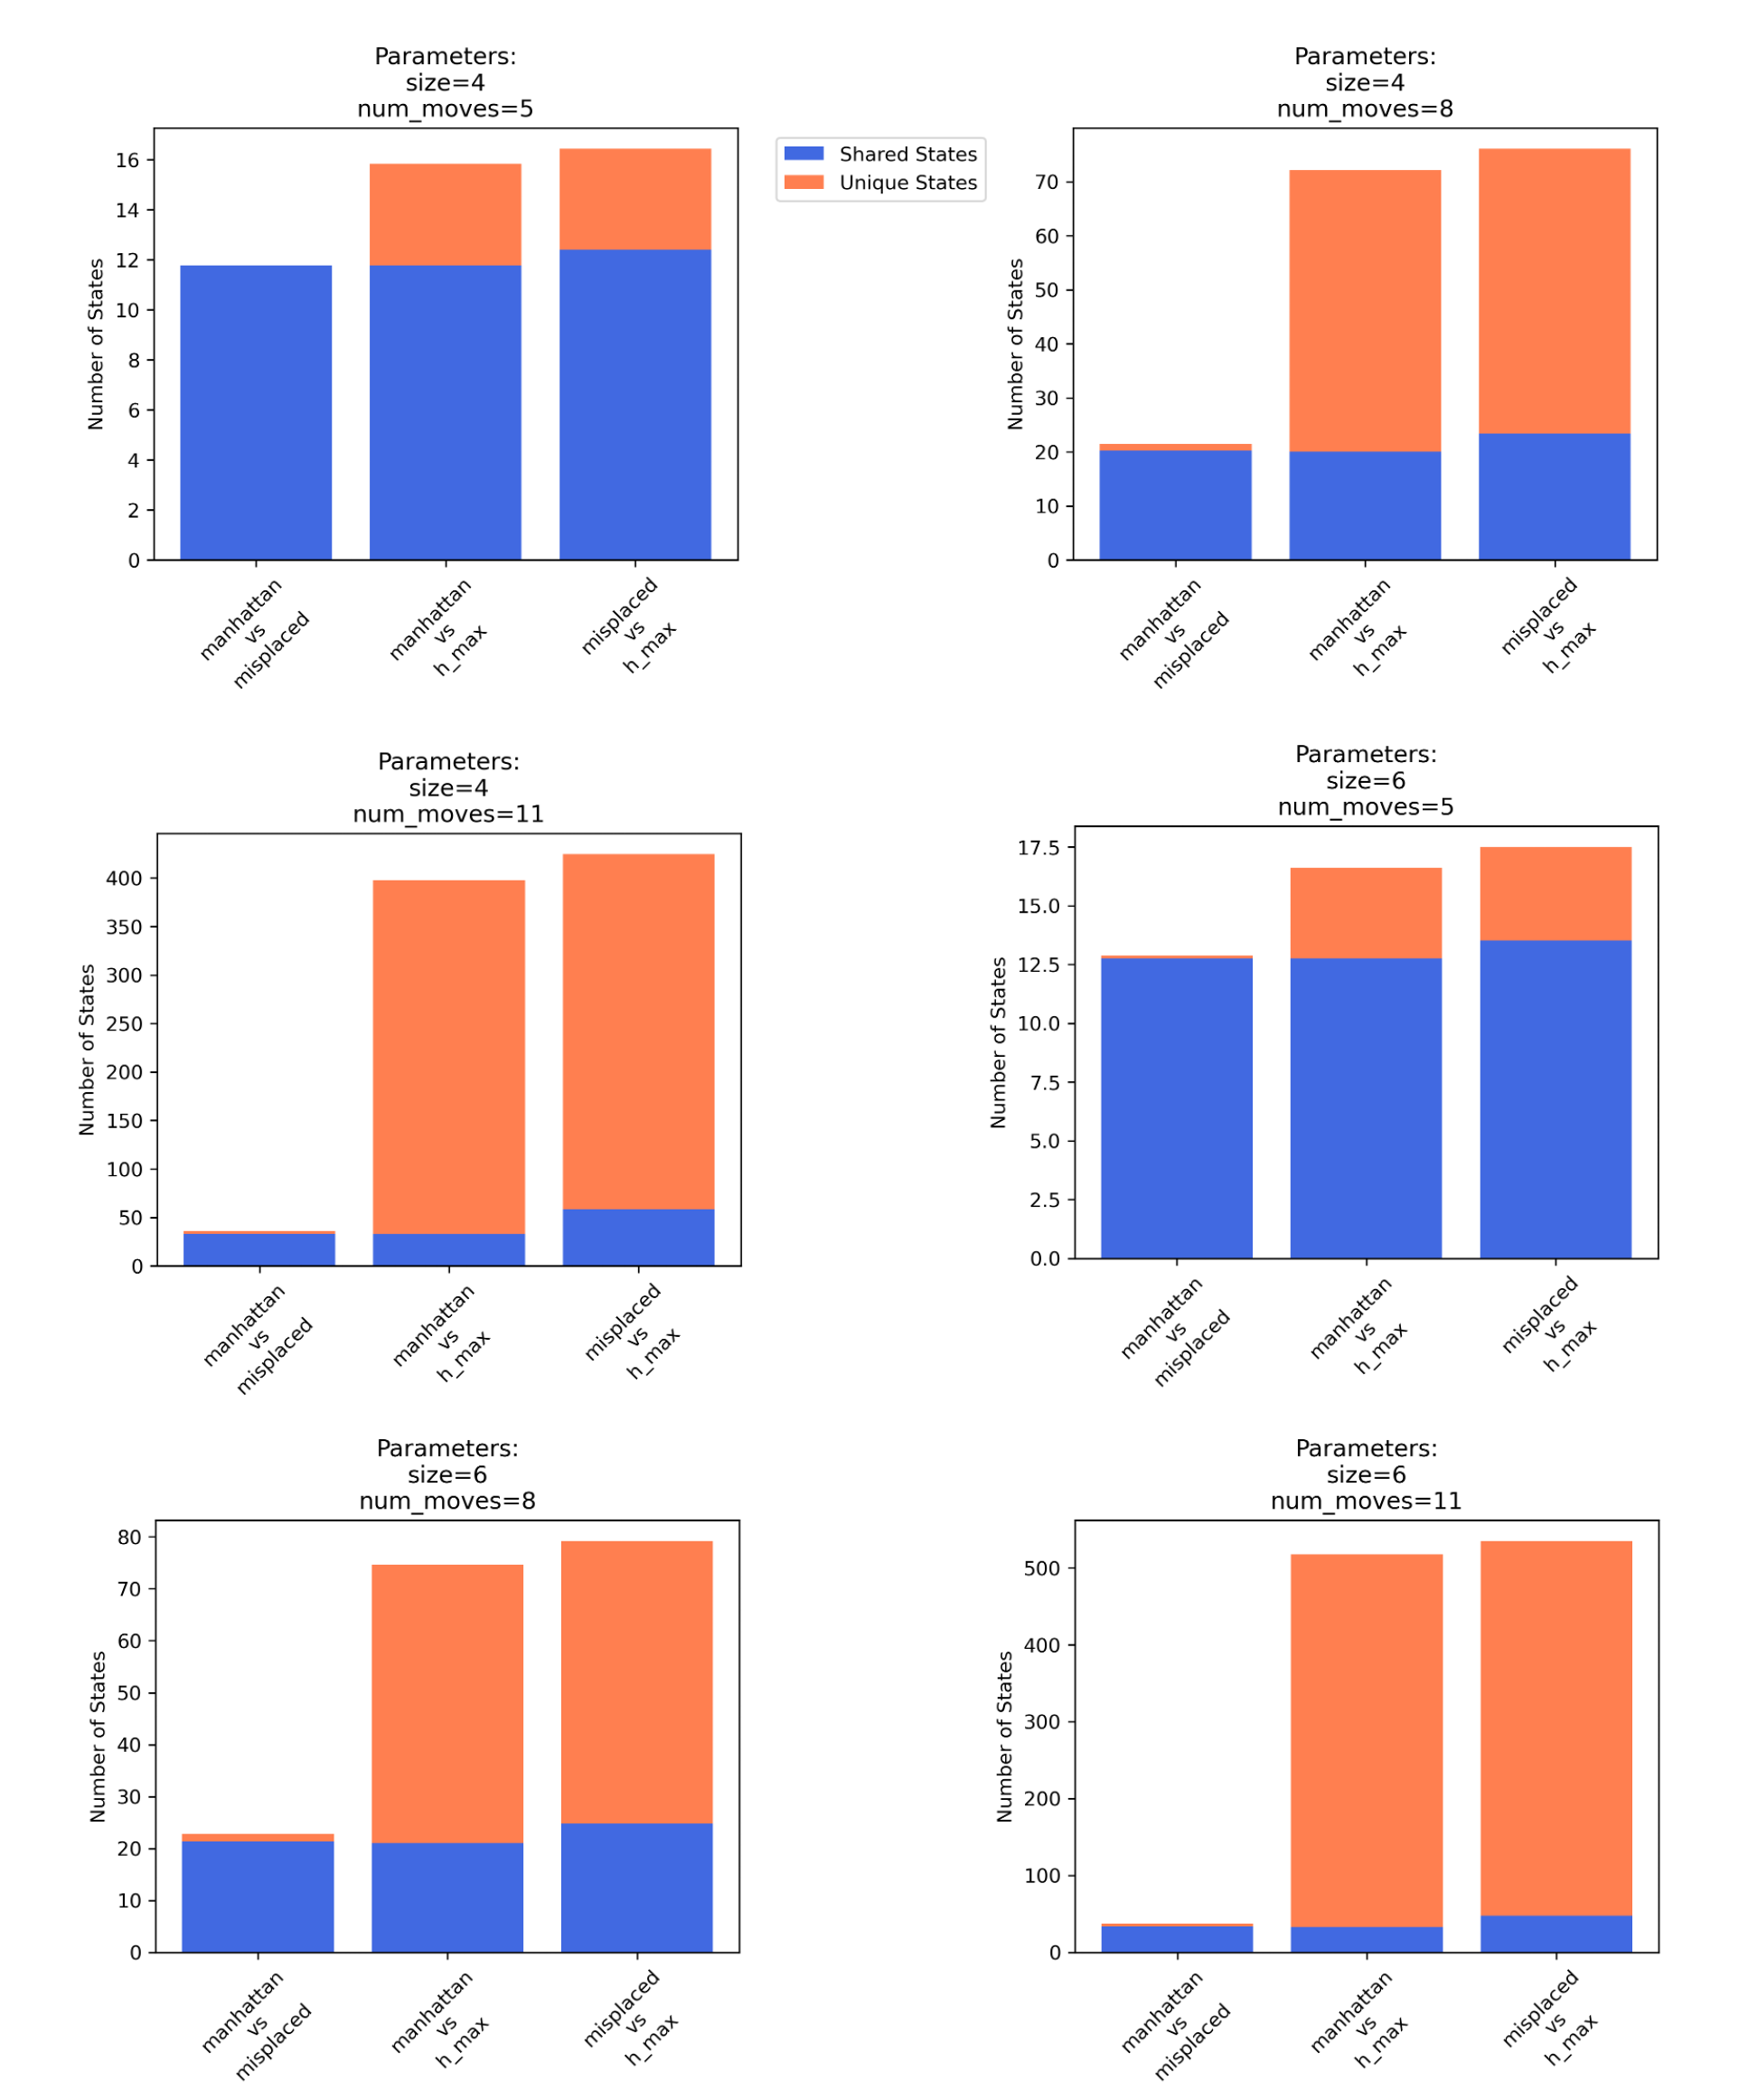
\includegraphics[width=\textwidth]{plots/sliding_puzzle_state_overlap_2.png}
    \end{minipage}
    \caption{Overlap of states expanded using different heuristics, on samples of varying parameters in Block-World and Sliding-Puzzle instances.}
    \label{fig:heuristic-overlap}
\end{figure*}

\begin{figure*}[ht]
    \centering
    \begin{minipage}{0.57\textwidth} % Two-thirds width
        \centering
        \caption*{Opened Nodes Order Difference in Blocks-World}
        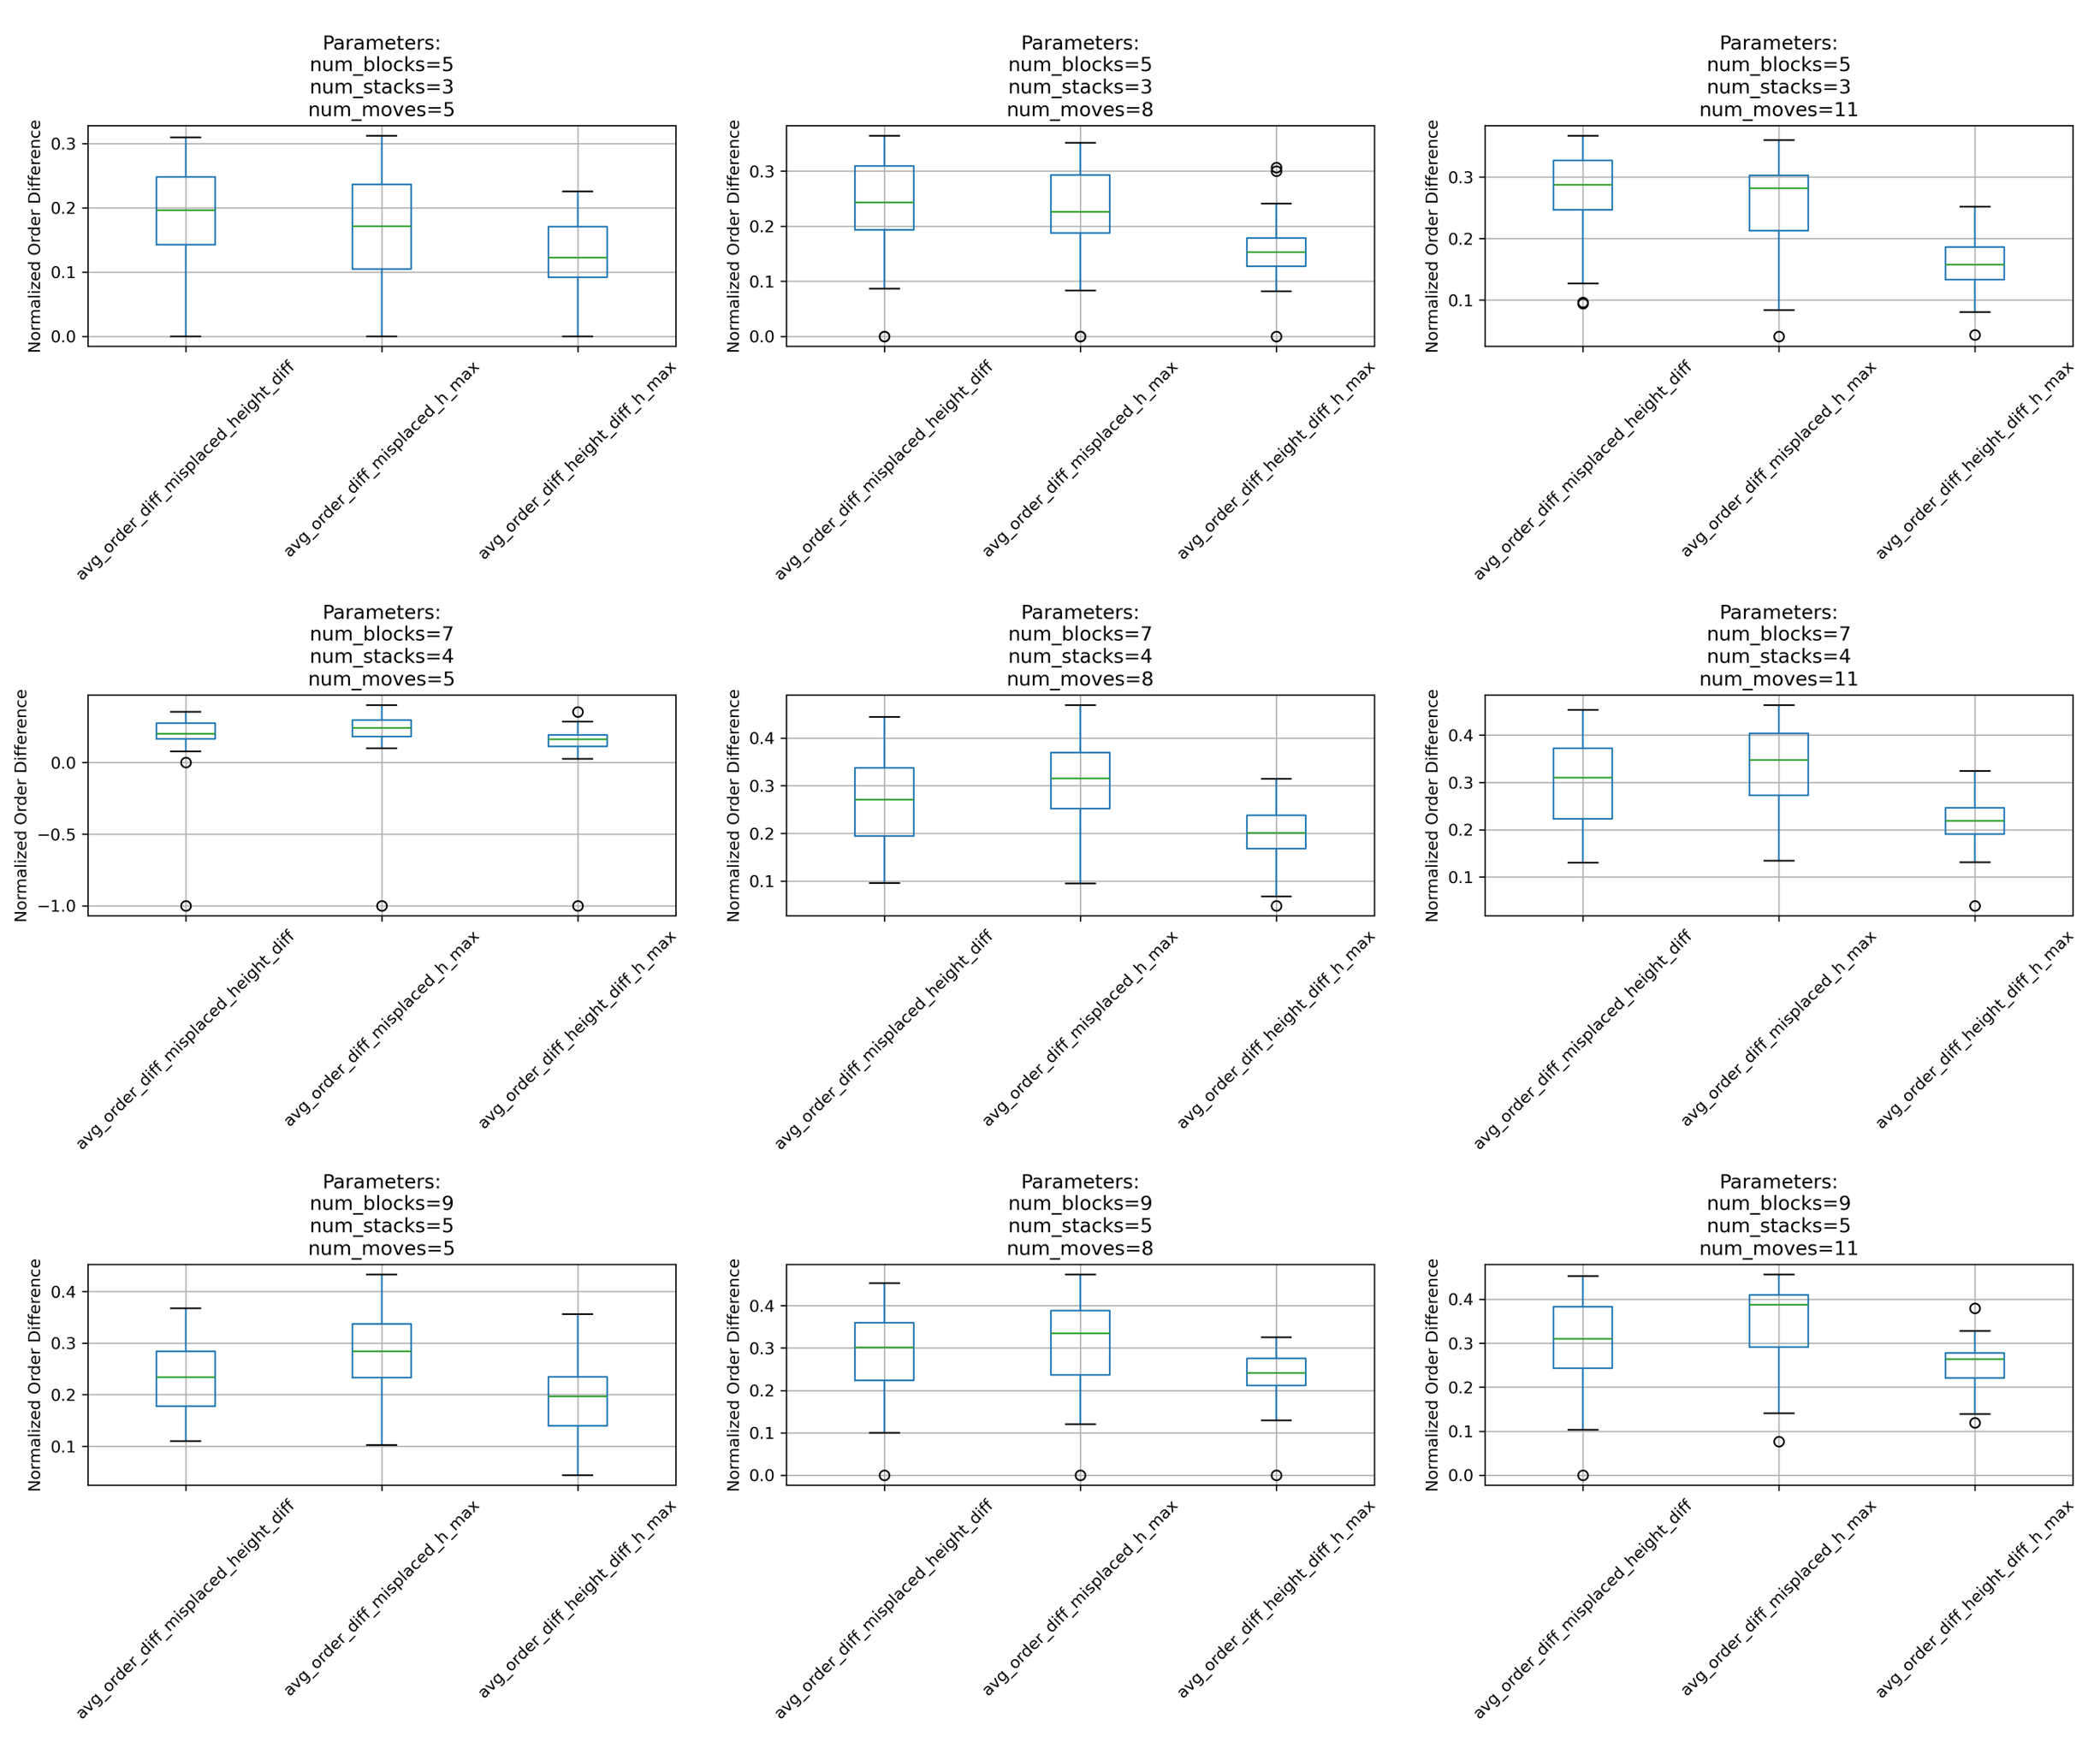
\includegraphics[width=\textwidth]{plots/blocks_world_order_differences_2.png}
    \end{minipage}%
    \hfill
    \begin{minipage}{0.39\textwidth} % One-third width
        \centering
        \caption*{Nodes Order Difference in Sliding-Puzzle}
        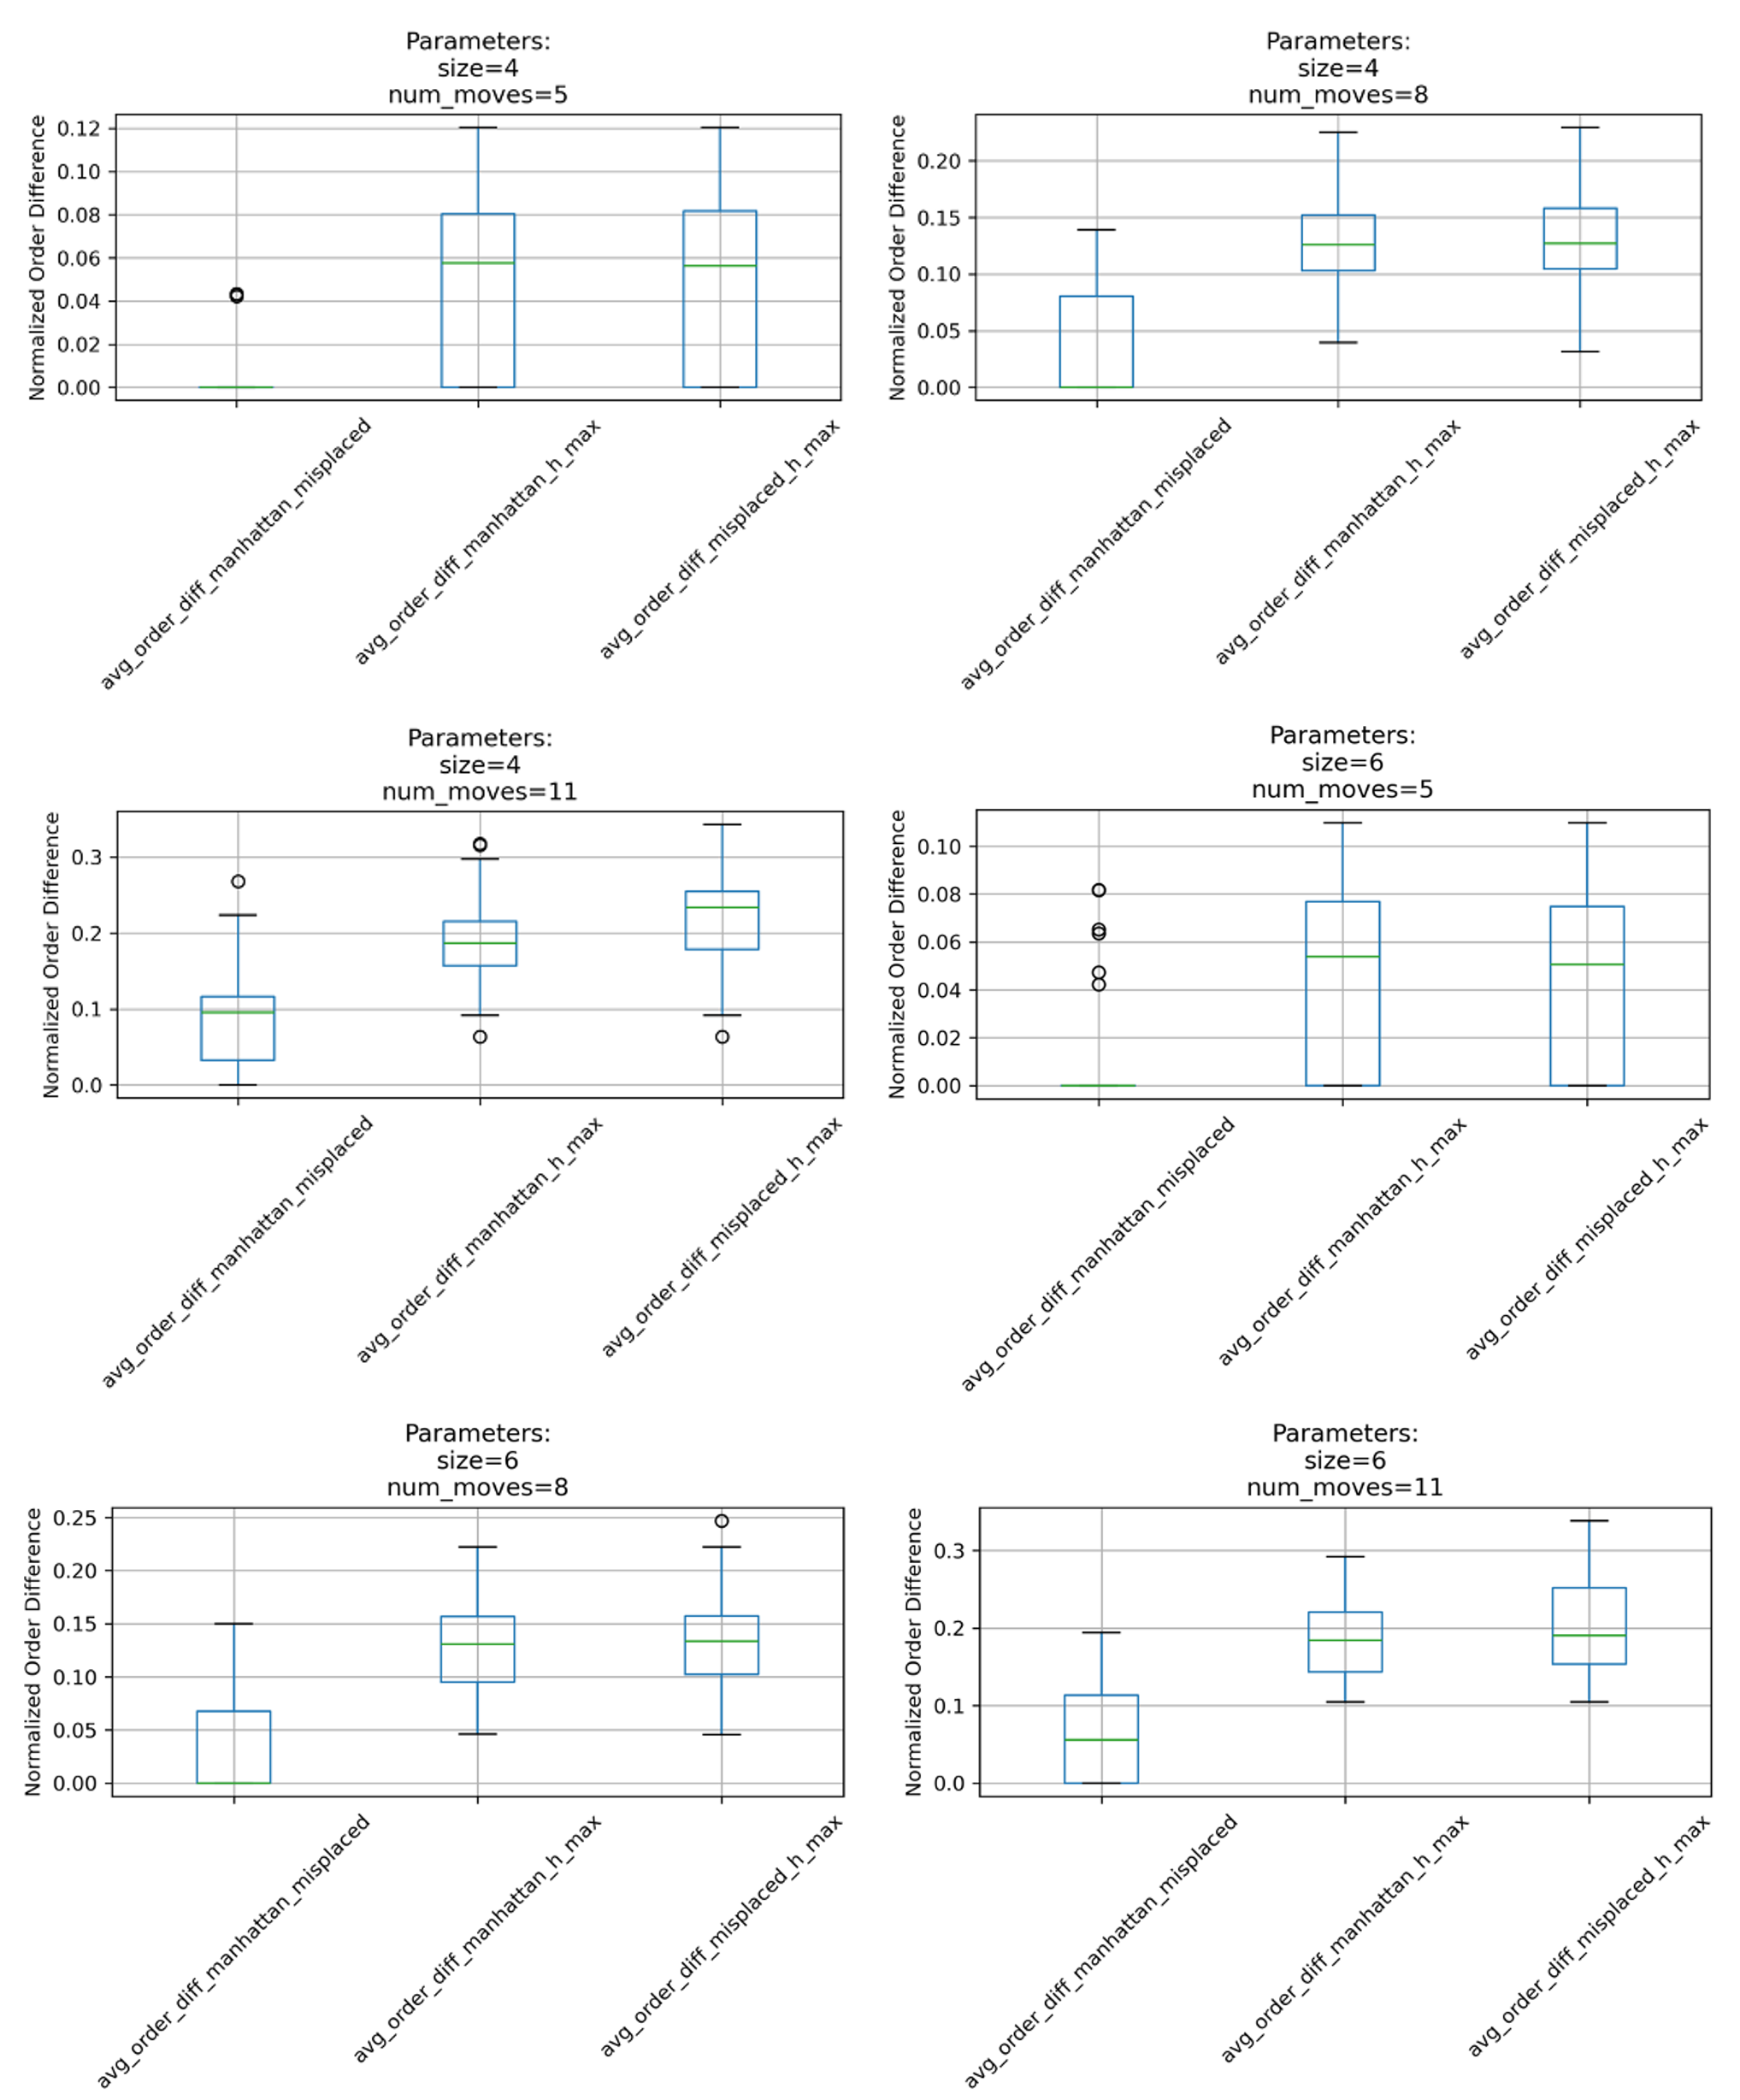
\includegraphics[width=\textwidth]{plots/sliding_puzzle_order_differences_2.png}
    \end{minipage}
    \caption{Normalized differences in node expansion order between different heuristics, calculated by Equation~\ref{eq:order-diff},on samples of varying parameters in Block-World and Sliding-Puzzle instances.}
    \label{fig:heuristic-order}
\end{figure*}

\subsection{Dataset Generation}

The key to training effective GNN models for search progress estimation lies in having a diverse and representative dataset of search graphs. We created a comprehensive dataset by implementing and running A* search on two distinct planning domains, Blocks-World and Sliding-Puzzle, each with three different heuristic functions.

For the Blocks-World domain, we implemented two domain-specific heuristics. The misplaced blocks heuristic ($h_{\text{misplaced}}$) counts blocks not in their goal positions, providing a quick but non-admissible estimate - since each misplaced block may require multiple moves. The height difference heuristic ($h_{\text{height}}$) sums absolute differences between current and goal stack heights divided by 2, offering an admissible but sometimes uninformative estimate - when stack heights match but blocks are misplaced.

Likewise, we implemented two heuristics specific to Sliding-Puzzle domain. The Manhattan distance heuristic ($h_{\text{manhattan}}$) sums the minimum vertical and horizontal moves needed for each tile, providing an admissible and computationally efficient estimate. The misplaced tiles heuristic ($h_{\text{misplaced}}$) counts tiles not in their goal positions, offering a quick but less informative estimate compared to Manhattan distance.

For both domains, we implemented the general heuristic $h_{\max}$. First, it constructs a relaxed planning graph by ignoring delete effects. The heuristic then computes costs layer by layer: each proposition in layer $i+1$ gets the minimum cost among all actions achieving it plus their precondition costs from layer $i$. Action costs are determined by the maximum cost among their preconditions plus 1. This process continues until reaching a fixed point or encountering all goal propositions, with the final $h_{\max}$ value being the maximum cost among the goal propositions. This provides a more sophisticated admissible estimate by capturing action dependencies, though at higher computational cost.

We generated problem instances with varying parameters to ensure good coverage of the problem space. For Blocks World, we varied the number of blocks (5-10), number of stacks (3-5), and solution depth (7-15 moves). For Sliding Puzzles, we generated boards of different sizes (5x5 to 9x9) with varying solution depths (7-15 moves). For each parameter combination, we generated 200 random problem instances.

For each problem instance, we ran A* search with all three domain-specific heuristics, recording detailed information about the search process. Each node in the resulting search graphs contains:
\begin{itemize}
    \item Search featuresas described in \nameref{para:learning-to-estimate}.
    \item Search trajectory information (parent node, children count).
    \item The desired prediction - search progress ($\frac{\text{serial number}}{\text{total nodes}}$).
\end{itemize}

The raw dataset contains approximately 2.9GB of search graphs across both domains. Importantly, while these graphs originate from different domains and heuristics, they share a common structure and feature set that makes them domain-agnostic from the model's perspective. Each graph represents a general search trajectory with standardized node features and connectivity patterns, allowing us to treat them as a unified collection of search behaviors rather than domain-specific examples.

\subsection{Dataset Pruning}

To make the dataset more practical for GNN training and to better simulate real-world scenarios, we implemented a two-stage pruning strategy. First, we filtered out graphs with more than 15,000 nodes to manage computational complexity. Second, we applied a dynamic pruning approach where for each remaining graph, we randomly selected a threshold $t \in \{0.3, 0.5, 0.7\}$ and kept only nodes with $\frac{\text{serial\_number}}{\text{total\_nodes}} < t$.

This second pruning stage is particularly important, as it simulates real-world scenarios where we must estimate search progress only with partial graph information. It forces our model to learn from incomplete search trajectories, making it more robust for practical applications where we don't have access to the full search graph. 

Without this pruning, we hypothesize that the models would trivially learn to compute progress by finding the maximum serial number through message passing and simply dividing each node's serial number by this maximum. 

Each graph maintains parent-child relationships between nodes, representing the actual search tree structure explored by A*. When pruning nodes, we carefully preserve edge connections between remaining nodes to maintain the graph's structural integrity. This preservation of structural information, even in pruned graphs, is crucial for our GNN-based approach, differentiating it from previous sequence-based methods.

\paragraph{The final processed dataset} consists of:
\begin{itemize}
    \item Blocks-World: 7312 graphs averaging 2519 nodes per full search graph.
    \item Sliding-Puzzle: 4633 graphs averaging 495 nodes per full search graph.
\end{itemize}


\subsection{Diversity Analysis}

To validate the diversity of our dataset, we conducted a comprehensive heuristic comparison study. This analysis revealed significant differences in search behavior across heuristics, which is crucial for the generalizability of the model. 

We compared three main aspects of search behavior across different heuristics: the number of nodes expanded, state space overlap, and similarity of exploration order.
Our analysis shows the number of nodes expanded varies considerably between heuristics for the same problem instances (Appendix~\ref{fig:heuristic-expanded}). Notably, Figure~\ref{fig:heuristic-overlap} demonstrates limited state space overlap between different heuristics, confirming that each heuristic explores the search space differently. 

Additionally, Figure~\ref{fig:heuristic-order} indicates that even among the overlapping nodes between the search spaces induced by different heuristics, there is a significant difference in their relative exploration order. Specifically, for each shared state $s$ between heuristics $h_1$ and $h_2$, we calculated a normalized order difference:
\begin{equation}\label{eq:order-diff}
    \text{Order Diff}(s) = \left|\frac{N_1(s)}{\max(N_1)} - \frac{N_2(s)}{\max(N_2)}\right|
\end{equation}
where $N_i(s)$ is the serial number (expansion order) of state $s$ under heuristic $h_i$. 

The results show varying expanded states and orders of exploration, particularly among larger problem instances. This diversity in search behaviors ensures our dataset captures a wide range of search patterns and progress trajectories.

\section{Models} \label{sec:models}

Our implementation includes two distinct GNN architectures tailored for different application needs: a high-accuracy model optimized for performance and a lightweight version suited for resource-limited environments.

\subsection{Full-Scale Architecture}
The primary architecture, HeavyGNN, employs a multi-scale approach to capture both fine-grained node relationships and broader structural patterns in the search space. At its core, the model combines Graph Attention Networks (GAT) with Graph Convolutional Networks (GCN) in parallel processing streams. The GAT component uses multi-head attention mechanisms to identify important node relationships, while the GCN component captures neighborhood structures through weighted message passing. These parallel streams are combined through feature fusion, with layer normalization applied to maintain stable training dynamics.

The model begins with a two-layer input projection to map raw node features into a learned representation space. The main architecture consists of multiple GAT-GCN blocks, with residual connections added every two layers to facilitate gradient flow in deeper networks. Each layer operates with a hidden dimension of 256 and uses 4 attention heads in the GAT component. The prediction head processes the final node representations through multiple fully-connected layers with decreasing dimensions, incorporating dropout for regularization, before producing the final progress estimate.

\subsection{Lightweight Architecture}
LightGNN provides an efficient alternative designed for scenarios where computational resources are limited or rapid inference is required. This model simplifies the architecture by using only GCN layers with improved neighborhood aggregation, removing the computationally expensive attention mechanisms while maintaining essential features for effective learning.

The lightweight model shares the same input projection and basic structure as HeavyGNN but replaces the parallel GAT-GCN streams with pure GCN processing. It maintains the use of layer normalization and residual connections while reducing the overall parameter count and computational complexity. 

Both architectures share common training elements including dropout regularization (p=0.2), residual connections every two layers, and edge weight learning. The models are trained using AdamW optimizer with weight decay and a learning rate warmup schedule.

\section{Experiments}
In this section, we present empirical evaluations of our GNN-based approaches against traditional benchmarks, and analyze their generalization capabilities across domains.

\subsection{Performance Comparison}

\begin{table}[t]
    \centering
    \caption{Performance comparison of different approaches}
    \label{tab:performance}
    \begin{tabular}{|l|c|c|}
    \hline
    \textbf{Model} & \textbf{MSE} & \textbf{Inference Time}\\
    \hline
    VeSP & 0.1605 & \\
    VaSP & 0.0569 & \\
    PBP & 0.0379 & \\
    Random Forest & 0.0328 & \\
    HeavyGNN & 0.00193 & \\
    LightGNN & 0.00151 & \\
    \hline
    \end{tabular}
\end{table}


We evaluated our GNN models against four established benchmarks: Velocity-based Search Progress (VeSP), Vacillation-based Search Progress (VaSP), Path-based Progress (PBP). An additional benchmark for learning to estimate was selected to be a Random Forest (RF) model, similarity to \citet{sudry2022learning}.
The RF trained on $80\%$ of the available nodes with their associated features as single datapoints, with 100 estimators and a maximum depth of 10. The remaining $20\%$ of nodes were used for evaluation to avoid overfit.

The benchmark evaluations were conducted on a dataset of 11,751 filtered search trees, representing diverse problem instances across both domains. \gur{More details}

Table \ref{tab:performance} presents each approach's Mean Squared Error (MSE) on the full collection of nodes in the dataset. The traditional benchmarks showed varying performance levels, with VeSP achieving the worse score. The formula based benchmarks achieve an error magnitude of $10^{-1}$ down to $10^{-2}$, while the Random Forest model achieved the best performance with an MSE within the $10^{-2}$ range. 

Our GNN-based approaches significantly outperformed all benchmarks. Both HeavyGNN and LightGNN achieved an MSE of $10^{-3}$, an order of magnitude improvement over the best-performing Random Forest model. Notably, despite its simplified architecture, LightGNN showed superior performance, suggesting that the core graph structural information is more important than complex architectural features for this task.

The results also present the trade-off between quality of predictions and computational efficiency during inference time. \naomi{expand...}


\subsection{Cross-Domain Generalization}

\begin{table}[t]
    \centering
    \caption{Cross-domain generalization results}
    \label{tab:cross_domain}
    \begin{tabular}{|l|l|c|}
    \hline
    \textbf{Training Domain} & \textbf{Test Domain} & \textbf{MSE} \\
    \hline
    Blocks World & Sliding Puzzle & 0.00158 \\
    Sliding Puzzle & Blocks World & 0.00272 \\
    \hline
    \end{tabular}
\end{table}

To evaluate the models' ability to generalize across different problem domains, we conducted cross-domain experiments where models were trained on one domain and tested on another. Table \ref{tab:cross_domain} shows the results of these experiments.

The results show strong generalization capabilities, both within the $10^{-3}$ order of magnitude. 
However, the results contain some asymmetry, as the model trained on Blocks-World showed better generalization to Sliding-Puzzle problems compared to the opposite direction. This can be attributed to the larger size of the Blocks-World dataset compared to the Sliding-Puzzle dataset, which likely enables the model to learn more robust and generalizable features of search progress patterns.

These cross-domain results are particularly impressive when compared to the in-domain performance, showing only a modest degradation in accuracy when generalizing to unseen domains. This suggests that our GNN models are learning fundamental search progress patterns that transfer well across different problem types, rather than merely memorizing domain-specific features.

\section{Conclusions and Future Work}

In this work, we developed a graph neural network approach for predicting search progress in heuristic search algorithms. We created a comprehensive framework for generating and collecting search graphs from two classical planning domains, implementing multiple heuristics for each domain. Our results demonstrate that GNNs can effectively leverage the structural information in search graphs to provide significantly more accurate progress estimates compared to traditional methods, with our models achieving an order of magnitude improvement in prediction accuracy. Furthermore, the strong cross-domain generalization results suggest that GNNs can learn fundamental patterns in search behavior that transcend specific problem domains.

Several limitations outside of the scope of our project offer promising directions for future work:

\begin{enumerate}
    \item \textbf{Domain and Algorithm Coverage:} Our evaluation is currently limited to two classical planning domains (Blocks World and Sliding Puzzle) and a single search algorithm (A*). While these domains represent different types of search spaces, future work should evaluate and adapt the approach for a broader range of planning domains and search algorithms (e.g. GBFS, beam search). This would provide stronger validation of the method's generalizability and practical utility.
    
    \item \textbf{Scalability Challenges:} Our project faced computational limitations with larger problems that generate extensive search graphs, and was limited to search graphs with below 15,000 due to this. However, true planning problems can generate search graphs of much larger sizes, and those applications are most relevant for progress estimation.
    
    While our pruning strategies help manage this issue, they introduce a trade-off between information completeness and computational feasibility. Future research should explore hierarchical graph processing methods that could help overcome these scaling limitations, while preserving structural information at different granularities. This might include developing adaptive sampling strategies or hierarchical graph representations that can efficiently handle larger search spaces.
    
    \item \textbf{Limited Feature Utilization:} Our model focuses solely on progress estimation, potentially missing opportunities to leverage the rich structural information in search graphs. Future work could explore multi-task learning approaches, training the GNN to simultaneously predict multiple search characteristics (e.g., solution quality, remaining search depth, likelihood of finding a better solution). This could improve overall performance through shared feature learning and provide more comprehensive search guidance.
\end{enumerate}

% If you have citations, uncomment the following line
\bibliography{aaai24}

\clearpage
\appendix
\onecolumn

\section{Heuristic Comparison}
\label{app:heuristic-comparison}

\begin{figure*}[ht]
    \centering
    \begin{minipage}{0.57\textwidth} % Two-thirds width
        \centering
        \caption*{Number of Expanded Nodes in Block-World Instances}
        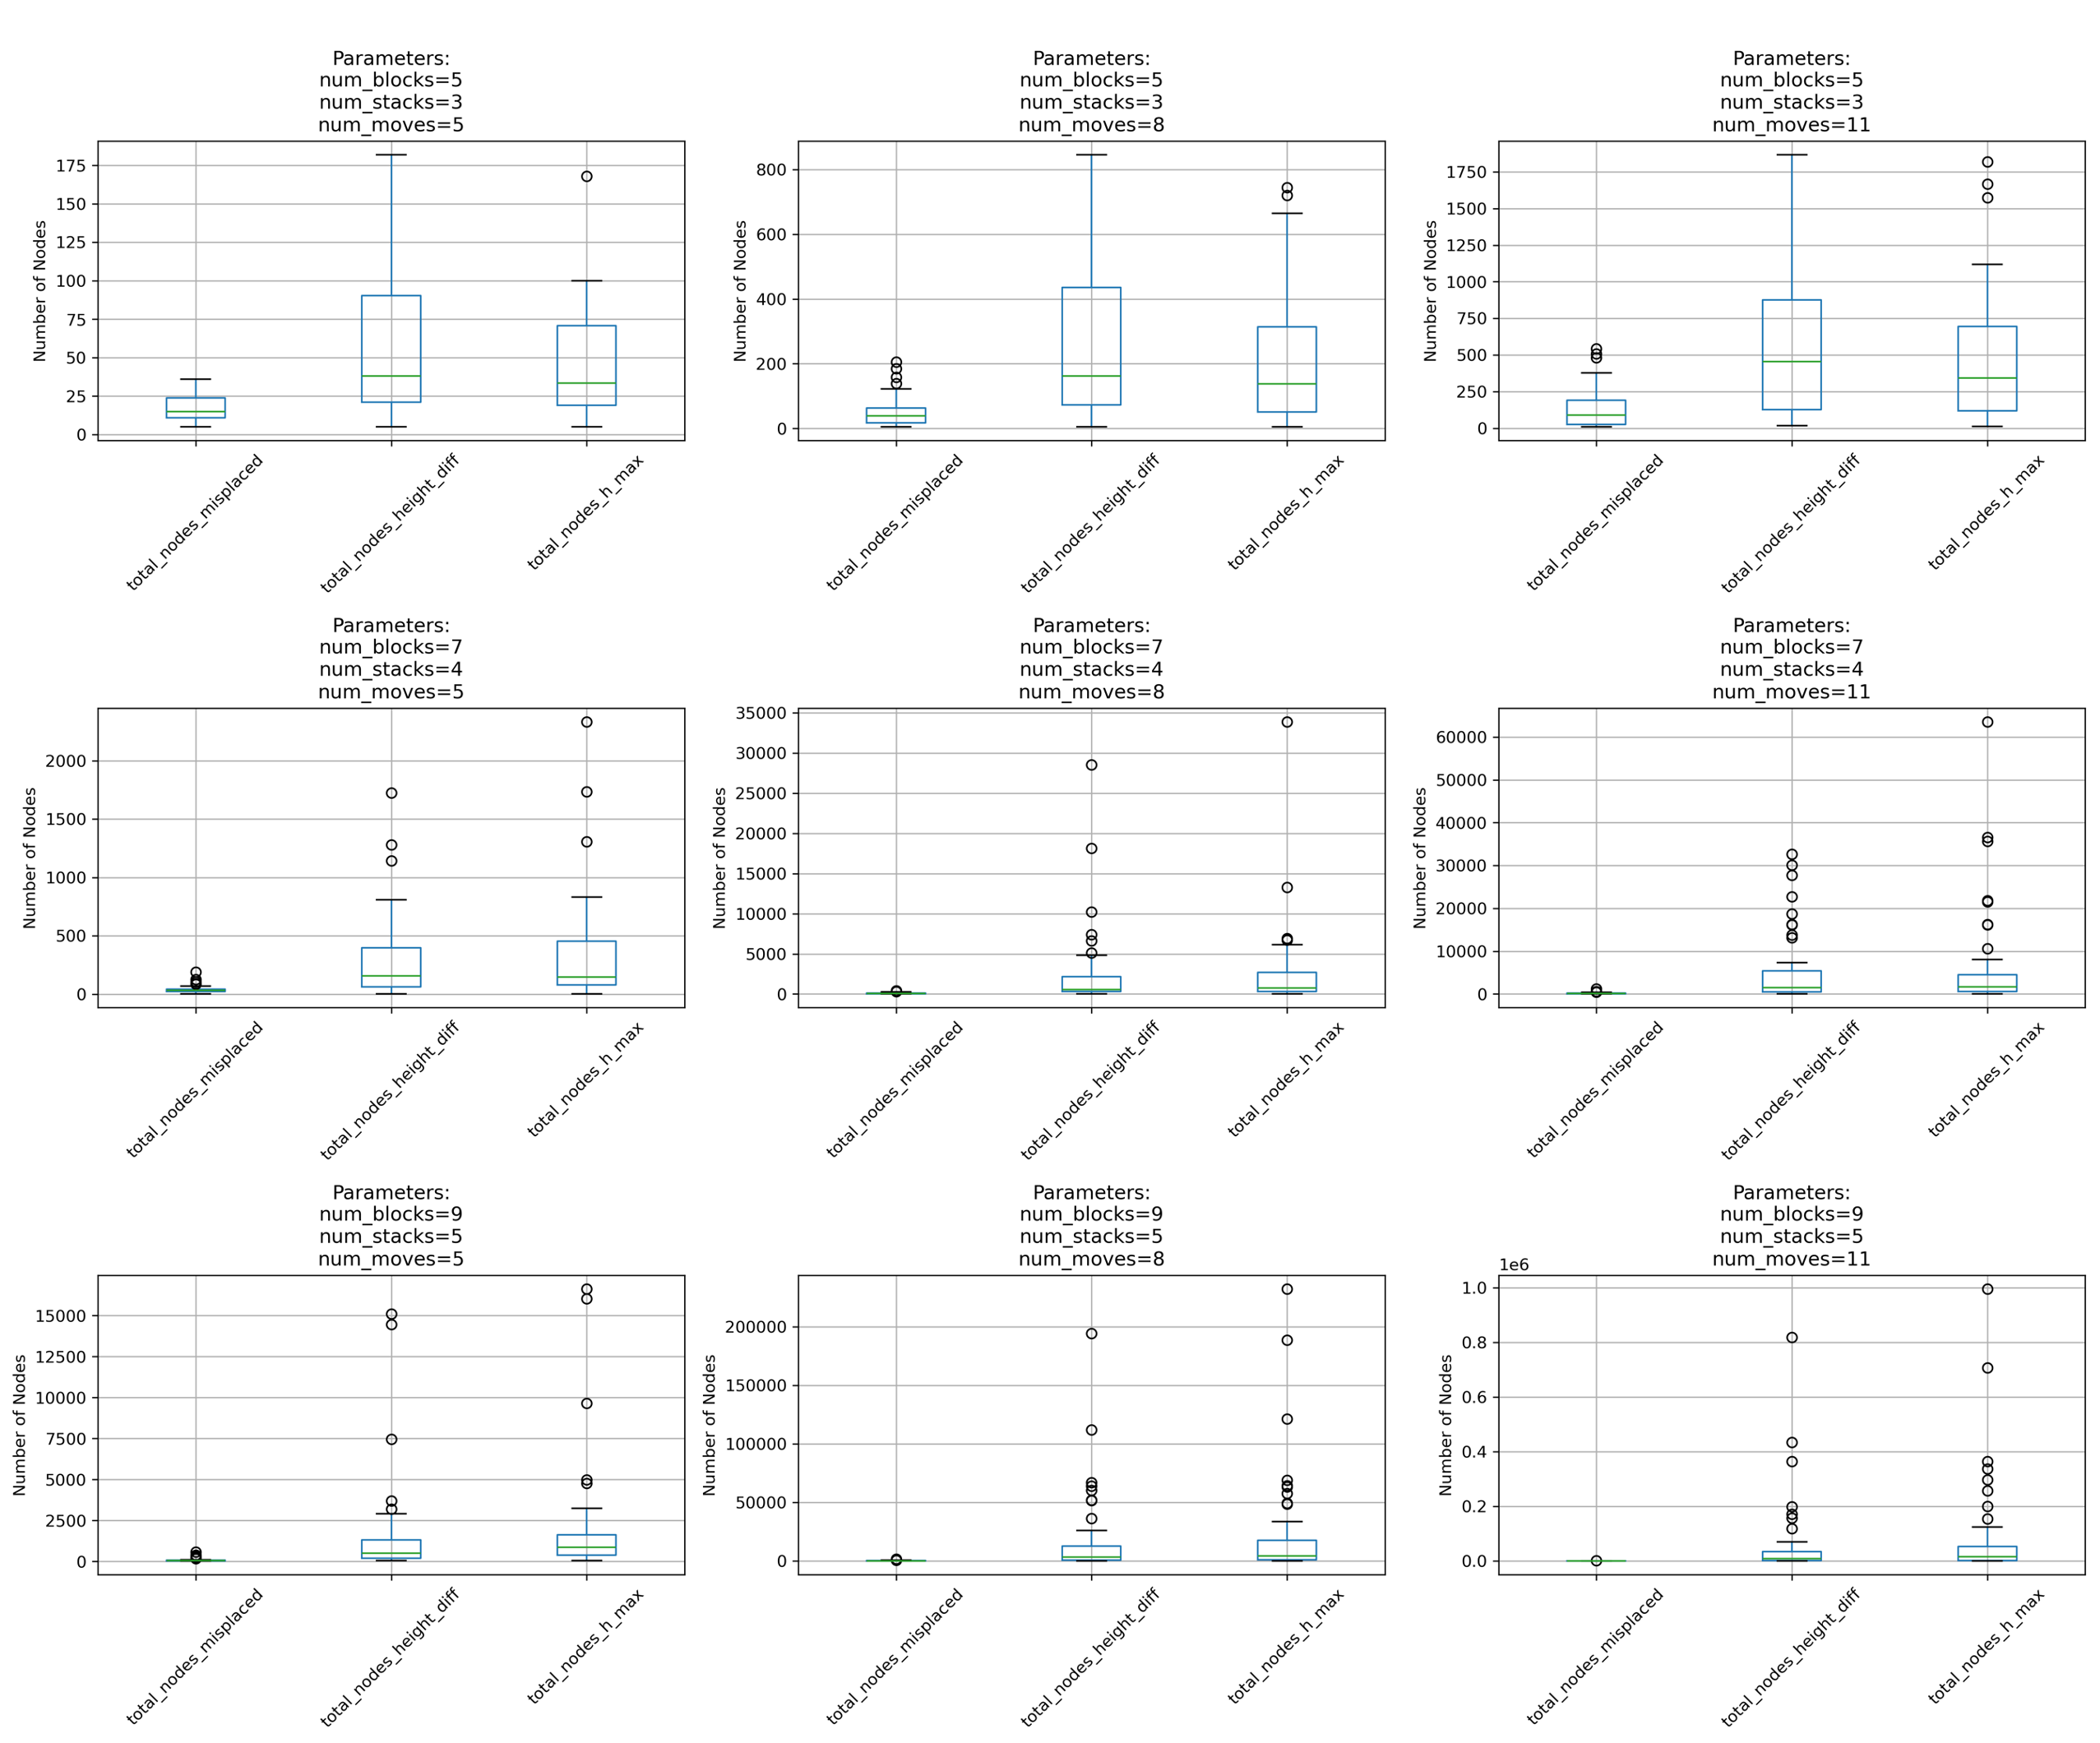
\includegraphics[width=\textwidth]{plots/blocks_world_nodes_expanded_2.png}
    \end{minipage}%
    \hfill
    \begin{minipage}{0.39\textwidth} % One-third width
        \centering
        \caption*{Number of Expanded Nodes in Sliding-Puzzle Instances}
        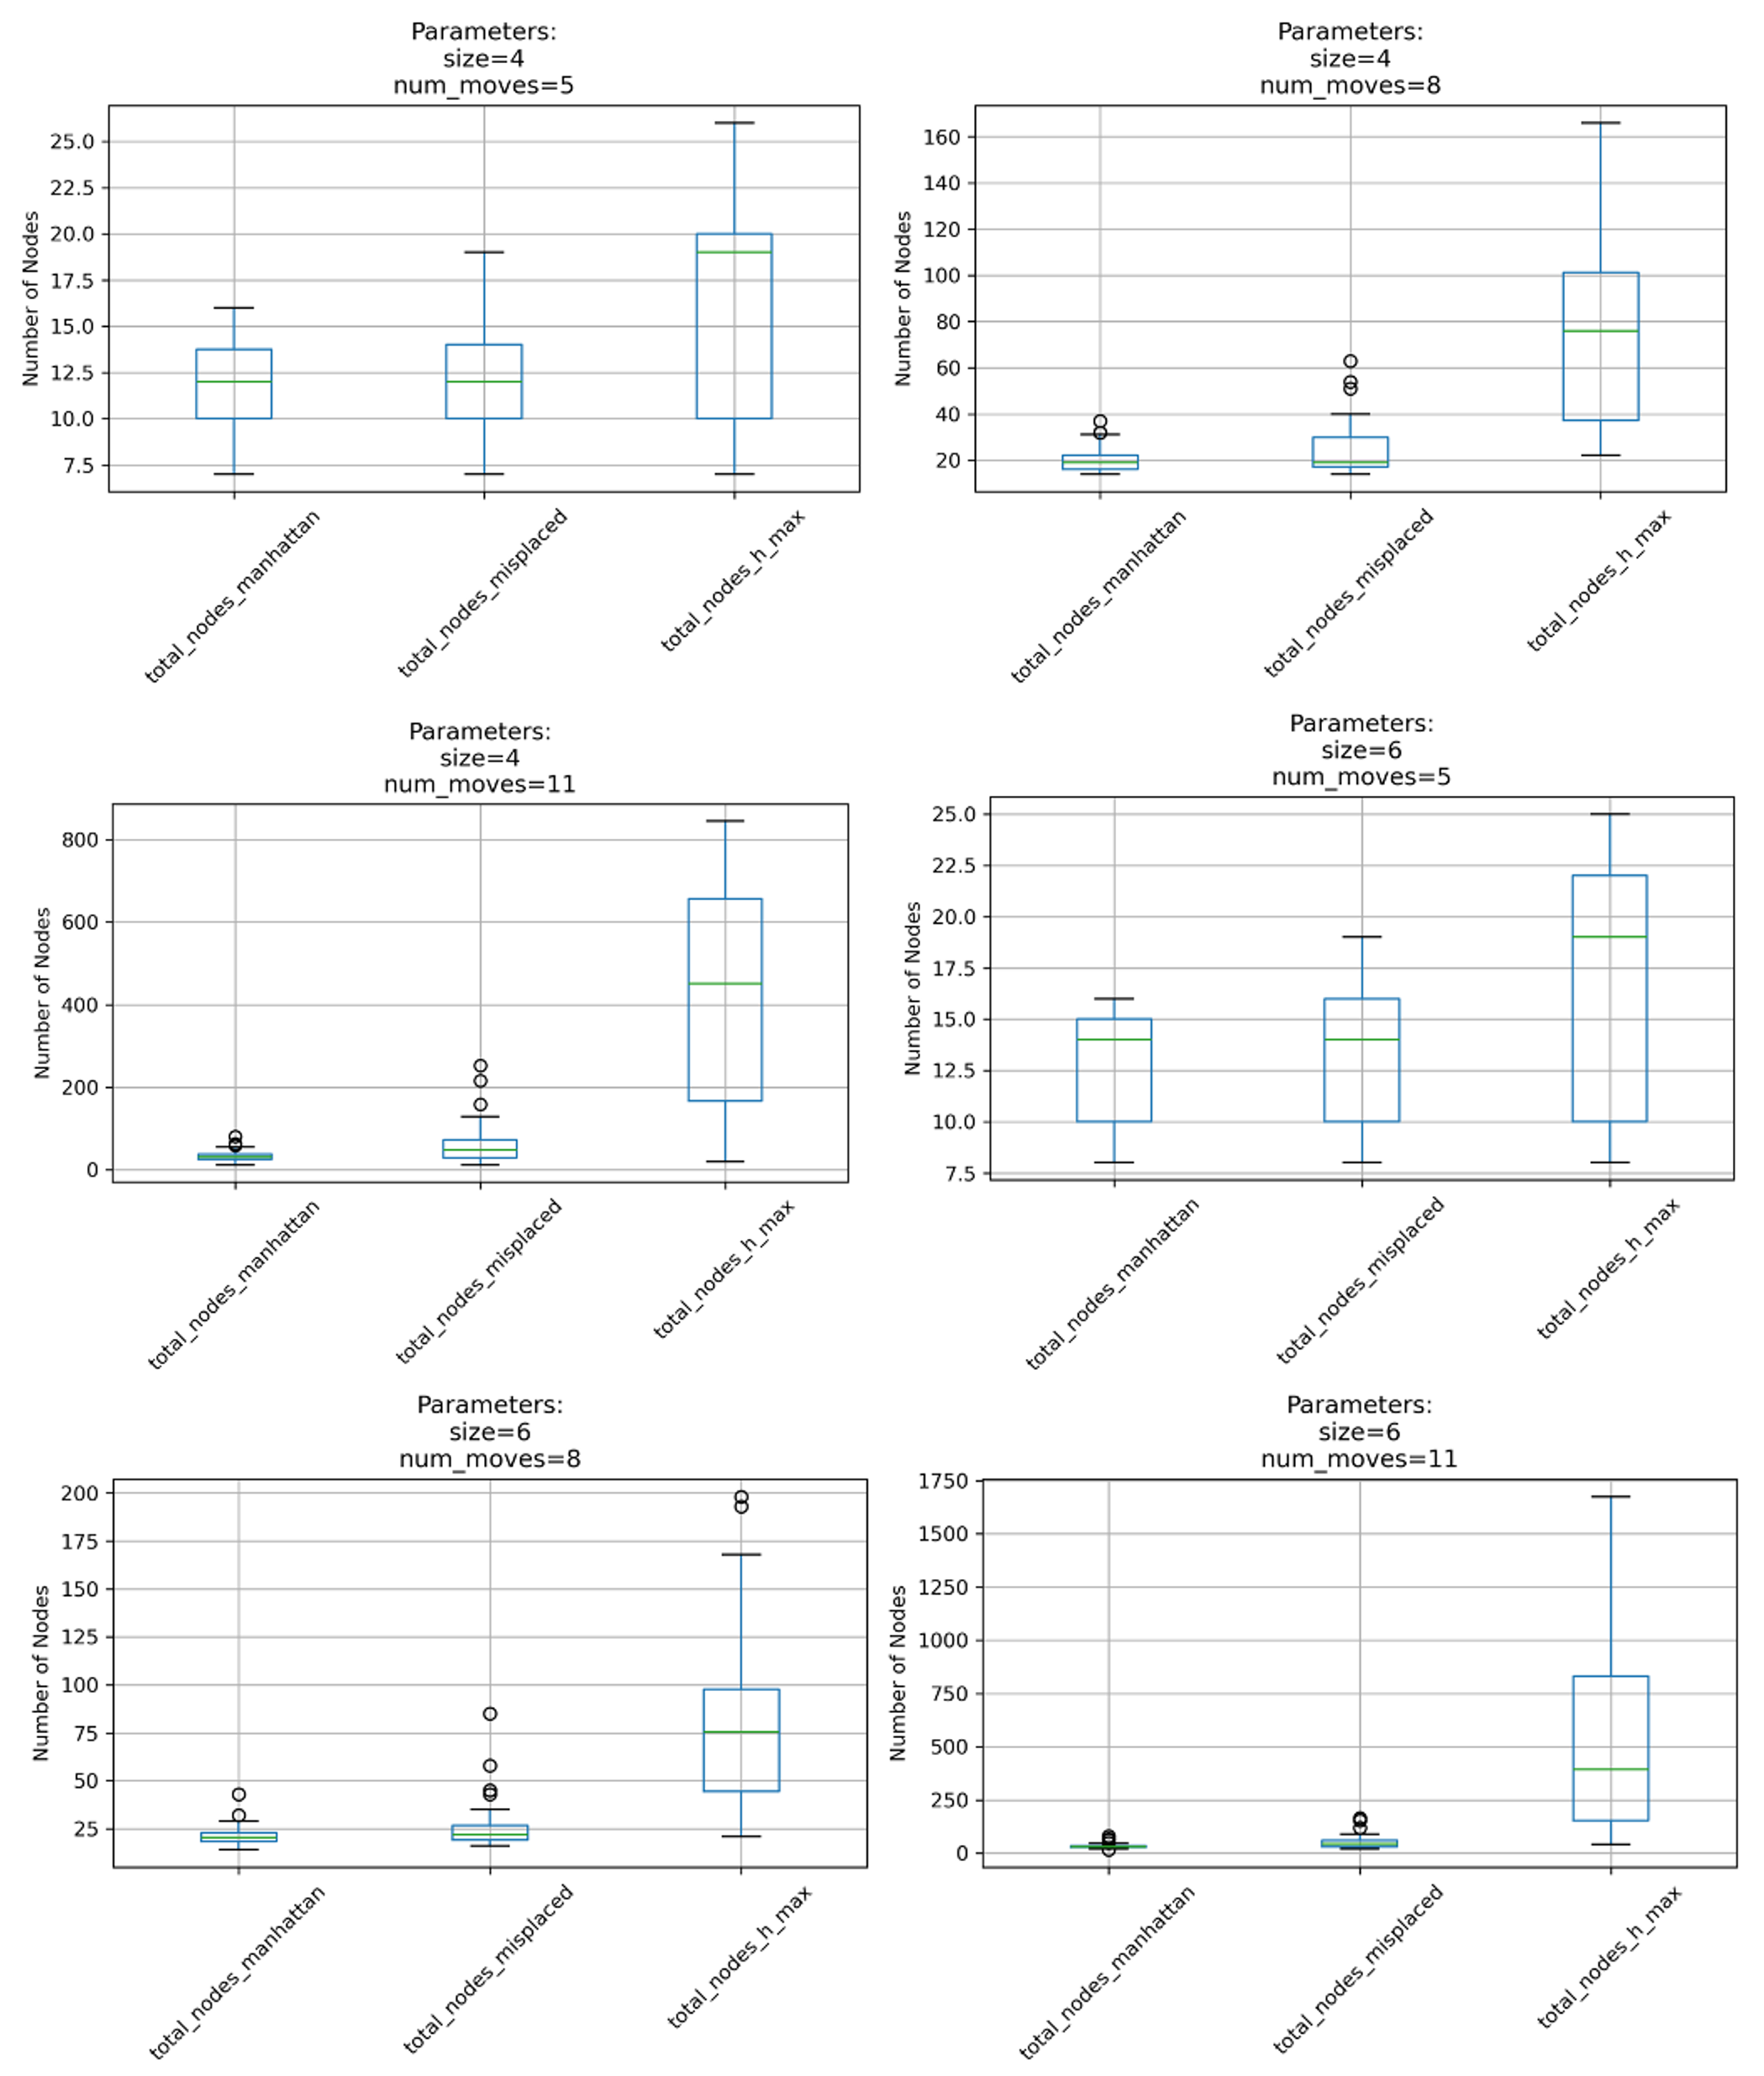
\includegraphics[width=\textwidth]{plots/sliding_puzzle_nodes_expanded_2.png}
    \end{minipage}
    \caption{Number of nodes expanded by different heuristics on samples of varying parameters in Block-World and Sliding-Puzzle instances}
    \label{fig:heuristic-expanded}
\end{figure*}



\end{document}